\documentclass[11pt,a4paper]{article}

\usepackage[a4paper, top=15mm, bottom=15mm, left=16mm, right=16mm]{geometry}
\usepackage[utf8]{inputenc}
\usepackage[T1]{fontenc}
\usepackage{lmodern}
\usepackage{graphicx}
\usepackage{amsmath,amssymb}
\usepackage{booktabs}
\usepackage{tabularx}
\usepackage{array}
\usepackage{float}
\usepackage{caption}
\usepackage{enumitem}
\usepackage{xcolor}
\usepackage{hyperref}

\hypersetup{
    colorlinks=true,
    linkcolor=blue!60!black,
    citecolor=blue!60!black,
    urlcolor=blue!60!black
}

\pagestyle{plain}
\linespread{0.96}
\setlength{\parskip}{2pt}
\setlength{\parindent}{0pt}
\setlength{\floatsep}{6pt}
\setlength{\textfloatsep}{8pt}
\setlength{\intextsep}{6pt}
\setlist{nosep, leftmargin=*}
\captionsetup{font=footnotesize, labelfont=bf, skip=3pt}

\begin{document}

% ==============================================================================
% TITLE BLOCK AND ABSTRACT (~0.5 PAGES)
% ==============================================================================
\begin{center}
    {\LARGE \bfseries Webcam-Based Strabismus (Squint) Screening and Vision Therapy System Using Dual-Eye Tracking\par}
    \vspace{6pt}
    {\small
    \textbf{Students:} J Gnana Teja Varma (Roll No: S20240010088) \quad | \quad V Sundhara Sai Ganesh (Roll No: S20240010250) \\
    \textbf{Project Type:} Bachelor of Technology Project (BTP) \quad | \quad \textbf{Evaluation:} Second Evaluation (Steps 1--3) \\
    \textbf{Project Mentor:} Dr.\ Pavan Kumar B N \quad | \quad \textbf{Repository:} \url{https://github.com/ganesh07365/eye-gaze-strabismus}
    \par}
\end{center}
\vspace{2pt}
\hrule
\vspace{6pt}

\begin{abstract}
\noindent Strabismus (ocular misalignment or squint) affects 2--4\% of children worldwide and causes irreversible amblyopia (lazy eye) and permanent loss of depth perception if undetected early. Conventional screening requires pediatric ophthalmologists, optical prism bars, and manual occluders, limiting accessibility in schools and rural clinics, while commercial infrared eye-trackers cost over \$1,000 and standard gaze CNNs merge both eyes into one coordinate. This project presents a software-only, real-time strabismus screening pipeline operating at 30~FPS on a standard 720p laptop webcam and CPU without discrete GPUs. Using MediaPipe 478-point landmarks, 3D head-pose decoupling, and a 11.7~mm anatomical iris ruler with spherical eyeball kinematics, the system tracks both eyes independently in clinical Prism Diopters ($\Delta\text{PD}$). Completed through Steps 1--3, it automates condition-gated Cover-Uncover, Alternate Cover, and 9-Cardinal Gaze tests, achieving 100\% diagnostic agreement across four clinical video categories and 6/6 accuracy on the triage verification suite.
\end{abstract}
\vspace{4pt}
\hrule
\vspace{6pt}

% ==============================================================================
% 1. INTRODUCTION (~0.5 PAGES)
% ==============================================================================
\section{Introduction}
\textbf{Problem Statement:} Strabismus is a binocular vision disorder in which the visual axes of both eyes fail to align simultaneously on a fixation target. Affecting approximately 2\% to 4\% of children globally~\cite{ref1}, untreated childhood strabismus causes the brain to suppress the deviating eye's cortical input to avoid double vision (diplopia). Over time, this suppression leads to permanent amblyopia (lazy eye) and irreversible loss of 3D stereopsis. Gold-standard clinical diagnosis relies on the Cover-Uncover Test, Alternate Cover Test (ACT), and 9-Cardinal Gaze Motility Exam performed by trained pediatric ophthalmologists using optical prism bars and manual occluders.

\textbf{Motivation:} In semi-urban and rural schools, specialist pediatric eye care is scarce, leaving subtle ocular deviations undetected beyond the critical period of visual plasticity. Consider a 6-year-old child with a subtle inward eye turn (esotropia): without routine screening, the condition may remain unnoticed until age 9, resulting in permanent visual impairment. An automated, 20-second screening session on an ordinary laptop webcam that measures a $26.5\,\Delta\text{PD}$ deviation and flags an immediate specialist referral can bridge this diagnostic gap at virtually zero hardware cost.

\textbf{Objectives:} The primary objective of this Bachelor of Technology Project (BTP) is to develop an accessible, software-only ocular screening and vision-therapy platform operating on a standard laptop webcam (720p, 30~FPS) without specialized infrared sensors or GPUs. Specifically, for Evaluation~2 (Steps 1--3), our goals are to:
\begin{enumerate}
    \item Track both eyes (OD and OS) independently in real time and convert pixel displacements into clinically interpretable Angular Degrees ($^\circ$) and Prism Diopters ($\Delta\text{PD}$).
    \item Automate condition-gated clinical protocols---Cover-Uncover, Alternate Cover, and 9-Cardinal Gaze Motility---with zero-lag automatic occlusion detection.
    \item Synthesize multi-protocol measurements into an explainable three-tier clinical triage verdict (\texttt{NORMAL}, \texttt{BORDERLINE}, \texttt{REFER}) protected by a physiological noise-floor guardrail.
\end{enumerate}

% ==============================================================================
% 2. LITERATURE REVIEW (~0.75 PAGES)
% ==============================================================================
\section{Literature Review}
Existing approaches to ocular alignment measurement and gaze estimation span clinical optometry tools, proprietary infrared hardware, deep appearance-based gaze networks, and static smartphone image classifiers. Table~\ref{tab:lit_review} summarizes five representative works alongside their clinical applicability and limitations.

\begin{table}[H]
\centering
\caption{Comparison of Related Clinical, Hardware, and Machine-Learning Approaches}
\label{tab:lit_review}
\footnotesize
\setlength{\tabcolsep}{4pt}
\begin{tabularx}{\textwidth}{@{}p{3.1cm}p{2.5cm}p{4.3cm}X@{}}
\toprule
\textbf{Work / Method} & \textbf{Modality} & \textbf{Key Capability} & \textbf{Limitation / Gap} \\
\midrule
Prism Cover Test (AAO PPP, 2022)~\cite{ref1} & Manual clinical exam & Gold-standard tropia, phoria, and $\Delta\text{PD}$ measurement & Requires specialist and prism bars; unsuitable for mass screening \\
Commercial IR Trackers (Tobii, EyeLink)~\cite{ref6} & Dedicated IR corneal reflection & Sub-degree binocular tracking precision & Costs \$1,000--\$5,000+; proprietary hardware limits deployment \\
MPIIFaceGaze / GazeCapture~\cite{ref4,ref7} & Deep CNN on RGB webcam & Appearance-based 3D gaze / screen cursor prediction & Merges both eyes into one target; blind to strabismus disparity \\
Smartphone Deep Screening~\cite{ref2,ref8} & Static 2D periocular photos & Automated squint detection from frontal eye photos & No 3D head-pose decoupling, occlusion gating, or motility matrix \\
I-VT Saccade \& MediaPipe~\cite{ref3,ref5} & RGB mesh + velocity threshold & Real-time 478-point landmarks and saccade segmentation & Not integrated into condition-gated $\Delta\text{PD}$ screening protocols \\
\bottomrule
\end{tabularx}
\end{table}

\textbf{Research Gap Addressed:} Standard AI gaze CNNs assume normal conjugate binocular vision: if a patient's left eye looks straight ($0^\circ$) while the right eye turns inward ($15^\circ$), averaging both eyes predicts a normal central fixation point and misses the squint completely. Conversely, static smartphone classifiers lack 3D head-pose compensation and cannot perform dynamic Cover-Uncover refixation tests or differentiate manifest tropia from latent phoria. To our knowledge, no open-source, CPU-only RGB webcam system independently tracks both eyes in physical Prism Diopters to automate condition-gated Cover-Uncover, ACT, and 9-Cardinal Gaze screening with multi-protocol clinical triage.

% ==============================================================================
% 3. RECAP OF PREVIOUS EVALUATION (~0.25 PAGES)
% ==============================================================================
\section{Recap of Previous Evaluation}
In \textbf{Evaluation~1}, we developed an initial webcam gaze-tracking prototype using MediaPipe facial landmarks and a custom ResNet-18 / GazeCNN model trained on the MPIIFaceGaze dataset~\cite{ref4}. That pipeline predicted a single binocular screen-cursor coordinate $(X, Y)$ (e.g., $X=540, Y=310$) with an average error of approximately $220\text{ px}$ and demonstrated a basic dwell-time interaction test.

During the Evaluation~1 review, our mentor (\textbf{Dr.\ Pavan Kumar B N}) advised pivoting away from generic cursor-control applications toward a high-impact clinical use case: \emph{pediatric strabismus screening and visual therapy}. Addressing this feedback required three foundational shifts: (1) replacing single-point screen gaze prediction with independent per-eye angular tracking (OD and OS), (2) introducing an anatomical $11.7\text{ mm}$ iris metric ruler to report ocular misalignment directly in clinical Prism Diopters ($\Delta\text{PD}$) rather than screen pixels, and (3) implementing automated Cover-Uncover, Alternate Cover, and 9-Cardinal Gaze protocols alongside a unified clinical triage engine (Steps~1--3).

% ==============================================================================
% 4. METHODOLOGY (~1 PAGE)
% ==============================================================================
\section{Methodology}
The screening pipeline is organized into three modular layers: Layer~1 (Perception and Dual-Eye Metric Engine), Layer~2 (Condition-Gated Clinical Protocols), and Layer~3 (Clinical Result and Triage Engine), as illustrated in Figure~\ref{fig:arch}.

\begin{figure}[H]
    \centering
    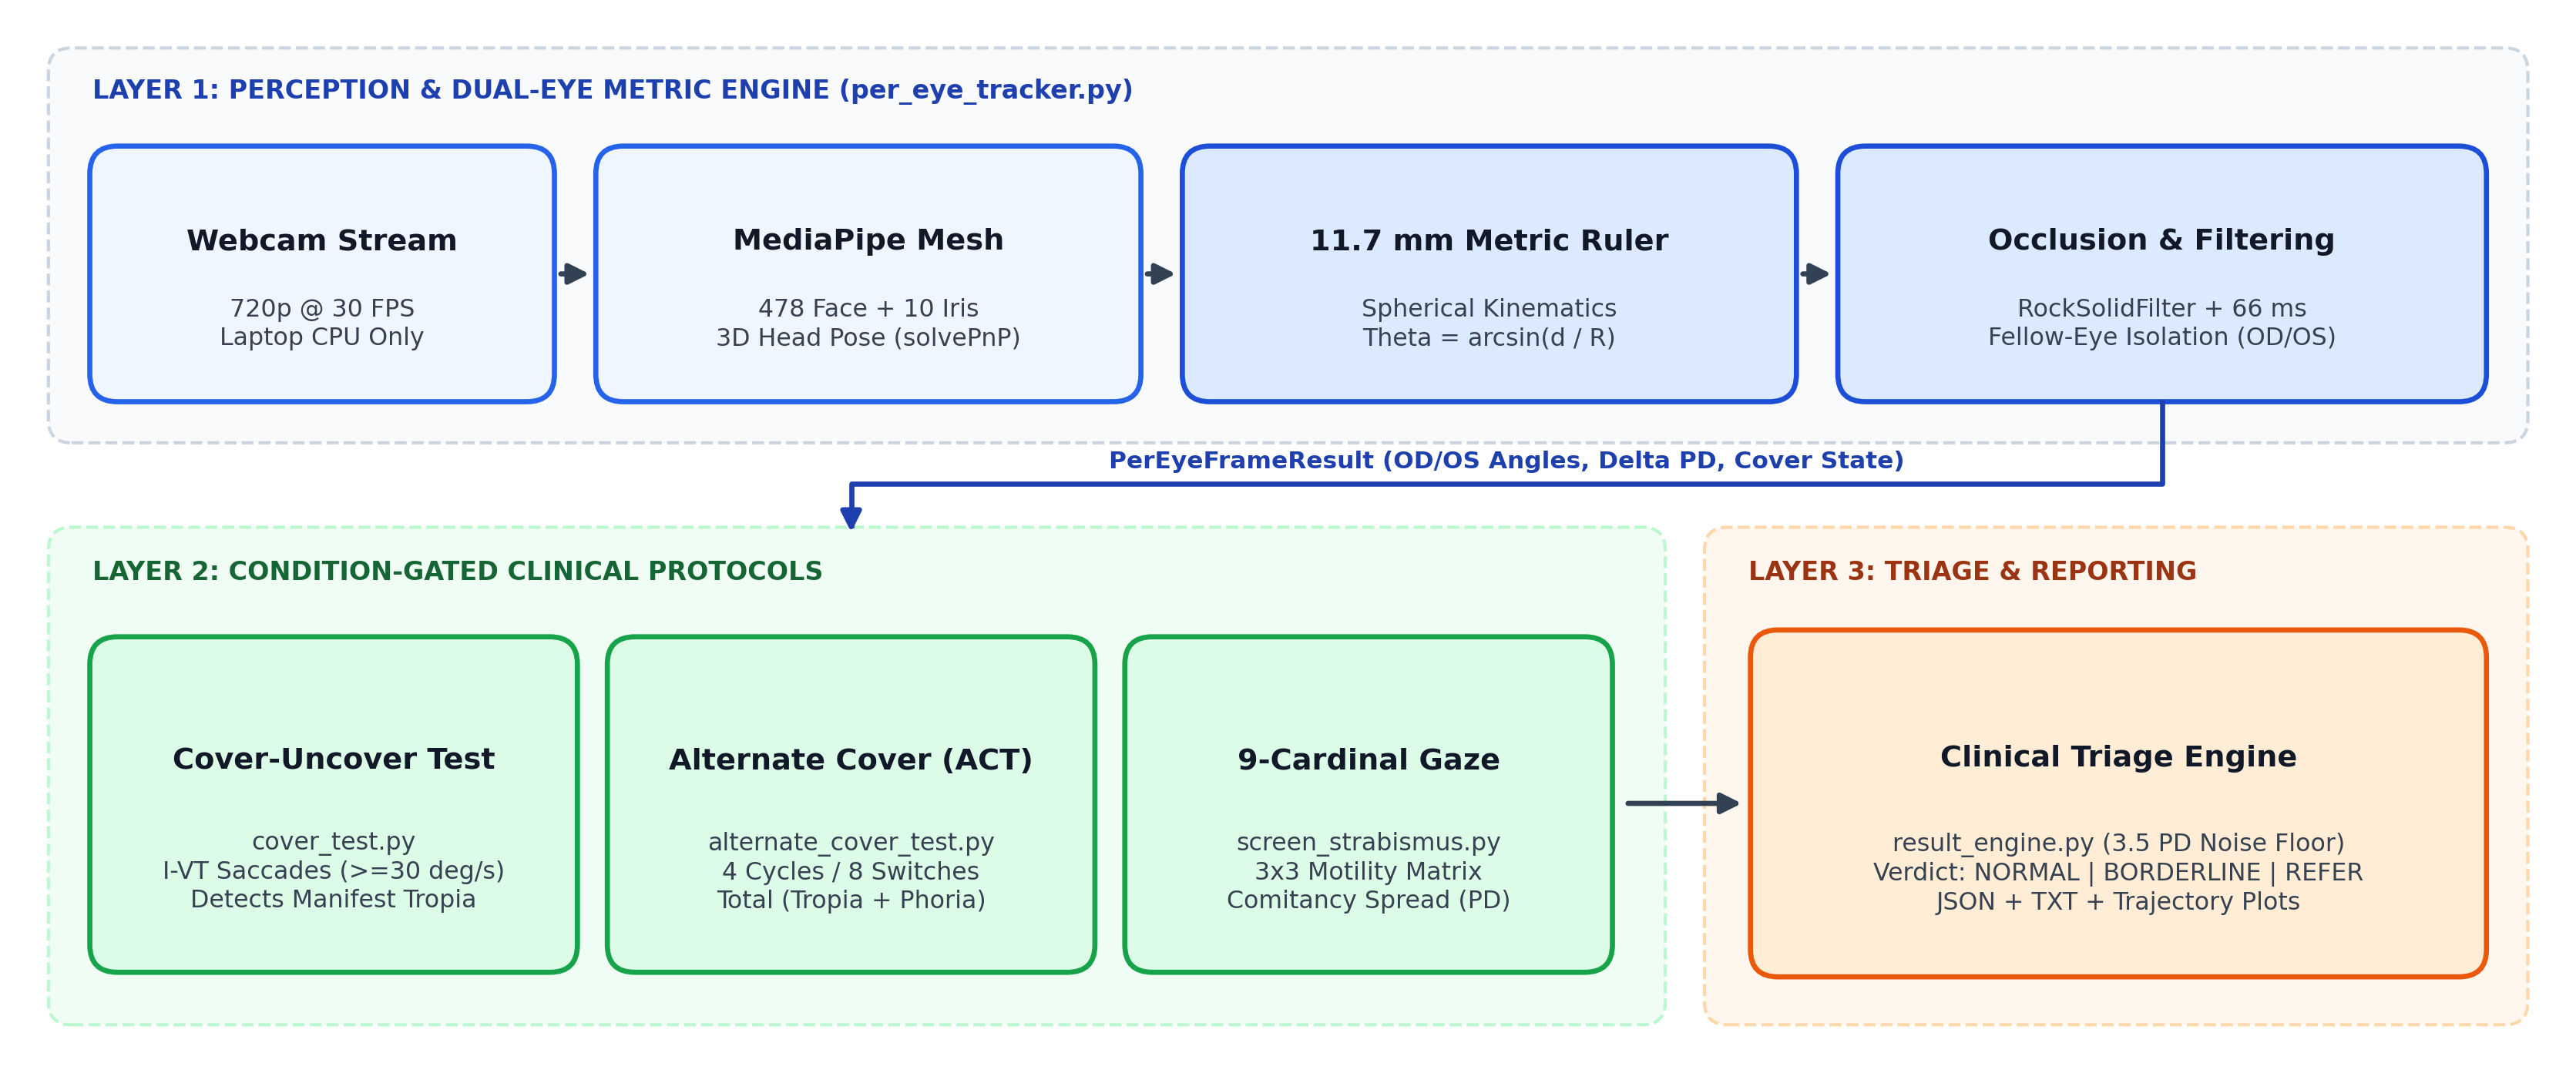
\includegraphics[width=0.90\textwidth]{figures/system_architecture.png}
    \caption{Three-layer system architecture connecting real-time webcam perception (\texttt{per\_eye\_tracker.py}), condition-gated clinical protocols, and automated triage reporting (\texttt{result\_engine.py}).}
    \label{fig:arch}
\end{figure}

\subsection{Anatomical Metric Scaling and Spherical Kinematics (Layer 1)}
Rather than relying on screen-dependent polynomial calibration, \texttt{per\_eye\_tracker.py} processes unmirrored RGB frames using Google MediaPipe's \texttt{FaceLandmarker} (478 facial mesh points and 10 iris boundary landmarks)~\cite{ref3} and extracts 3D head orientation $(\text{yaw}, \text{pitch}, \text{roll})$ from the facial transformation matrix via \texttt{solvePnP} alignment so head movements do not mimic eye rotation. For each eye independently (OD: right eye, OS: left eye), the horizontal iris diameter in pixels $w_{\text{iris}}$ is scaled against the invariant adult corneal diameter $D_{\text{iris}} = 11.7\text{ mm}$~\cite{ref1} to obtain a self-calibrating pixel-to-millimeter factor:
\begin{equation}
s = \frac{11.7\text{ mm}}{\max(w_{\text{iris}}, 1.0)} \quad (\text{mm/px})
\end{equation}
Projecting the iris displacement vector $\mathbf{d}_{\text{iris}}$ onto the eye's nasal ($\mathbf{u}_{\text{nasal}}$) and downward ($\mathbf{u}_{\text{down}}$) canthal axes yields physical displacements $(d_h, d_v)$ in millimeters. Using spherical eyeball kinematics with mean eyeball radius $R = 12.0\text{ mm}$, the eye rotation angles are computed as:
\begin{equation}
\theta_{\text{yaw}} = \arcsin\!\left(\text{clip}\!\left(\frac{d_h}{R}, -0.95, 0.95\right)\right), \qquad \theta_{\text{pitch}} = \arcsin\!\left(\text{clip}\!\left(\frac{d_v}{R}, -0.95, 0.95\right)\right)
\end{equation}
Because nasal coordinates point medially for both eyes, conjugate side gaze induces equal and opposite signs ($\theta_{\text{OD}} = -k$, $\theta_{\text{OS}} = +k$), canceling cleanly when summed. Inter-ocular misalignment in degrees and ophthalmic Prism Diopters ($\Delta\text{PD}$) is therefore:
\begin{equation}
\Delta\theta_H = \theta_{\text{OD,yaw}} + \theta_{\text{OS,yaw}}, \qquad \Delta\theta_V = \theta_{\text{OS,pitch}} - \theta_{\text{OD,pitch}}, \qquad \Delta\text{PD} = 1.7455 \times \Delta\theta
\end{equation}
where $\Delta\text{PD}_H > 0$ denotes esotropia (inward convergence) and $\Delta\text{PD}_H < 0$ denotes exotropia (outward divergence). Raw signals pass through \texttt{RockSolidFilter}, a 3-frame median filter coupled with an adaptive exponential moving average ($\alpha_{\text{still}} = 0.25$, $\alpha_{\text{move}} = 0.85$ above saccade threshold $0.4^\circ$) and deadband ($0.05^\circ$) to suppress webcam jitter while preserving sharp refixation saccades.

\subsection{Zero-Lag Occlusion Sensing and Condition-Gated Protocols (Layers 2--3)}
To automate cover testing without manual button presses, each eye crop is evaluated for physiological openness (palpebral aperture $\ge 0.13$, texture $\sigma \ge 8.0$, P90--P10 contrast $\ge 14.0$, mean luminance $\ge 35.0$) alongside hemispheric ROI brightness asymmetry ($|\Delta I_{\text{ROI}}| > 25$). A 3-frame majority vote yields occlusion states (\texttt{NONE}, \texttt{OD}, \texttt{OS}, \texttt{BOTH}) within $\sim 66\text{ ms}$. Built atop this tracker:
\begin{itemize}
    \item \textbf{Cover-Uncover Test (\texttt{cover\_test.py}):} A condition-gated state machine advancing only on verified positioning, central bullseye fixation, and fellow-eye occlusion. Our I-VT analyzer ($v \ge 30^\circ/\text{s}$)~\cite{ref5} extracts refixation amplitude, latency, and peak velocity to detect manifest tropia.
    \item \textbf{Alternate Cover Test (\texttt{alternate\_cover\_test.py}):} Enforces 4 alternating occlusion cycles (8 transitions, $2.0\text{ s}$ hold, $600\text{ ms}$ switch grace window) to break binocular fusion and quantify Total Dissociated Deviation ($\text{Tropia} + \text{Phoria}$) and Hering's Law symmetry.
    \item \textbf{9-Cardinal Gaze Matrix (\texttt{screen\_strabismus.py}):} Measures alignment and Bivariate Contour Ellipse Area (BCEA)~\cite{ref9} across 9 gaze targets, computing Incomitancy Spread ($\max \Delta\text{PD} - \min \Delta\text{PD}$) to distinguish comitant squint ($\le 5.0\,\Delta\text{PD}$) from paretic incomitancy ($> 8.0\,\Delta\text{PD}$).
    \item \textbf{Triage Engine (\texttt{result\_engine.py}):} Enforces a $3.5\,\Delta\text{PD}$ sensor noise floor, isolates latent phoria ($\max(0, \text{ACT} - \text{Manifest})$), and outputs \texttt{NORMAL}, \texttt{BORDERLINE}, or \texttt{REFER} with confidence scores and clinical flags.
\end{itemize}

\textbf{Why Geometric Modeling Over Black-Box CNNs:} Clinical screening requires transparent, physically grounded measurements in Prism Diopters that ophthalmologists can verify against prism bars, rather than opaque neural confidence scores that vary unpredictably under changing camera distances.

% ==============================================================================
% 5. IMPLEMENTATION DETAILS (~0.75 PAGES)
% ==============================================================================
\section{Implementation Details}
\textbf{Hardware and Software Stack:} The platform executes entirely on a consumer laptop CPU (integrated 720p webcam at $1280\times720$, $30\text{ FPS}$) with zero discrete GPU dependency. The software stack comprises Python~3.14, Google MediaPipe~0.10 (\texttt{face\_landmarker.task}), OpenCV~4.10, NumPy~2.x, Matplotlib~3.10 (headless Agg backend for diagnostic plots), and PyTorch for an auxiliary 5-class Siamese classifier (\texttt{DualGazeStrabismusNet} in \texttt{core/train\_strabismus\_net.py}) transferring convolutional weights from \texttt{gaze\_model\_p00.pth}.

\textbf{Datasets:} Dynamic screening protocols are evaluated against four ground-truth clinical benchmark videos in \texttt{diagnostics/samples/}: normal (\texttt{01\_normal.mp4}), inward squint (\texttt{02\_esotropia.mp4}), outward squint (\texttt{03\_exotropia.mp4}), and vertical squint (\texttt{04\_hypertropia.mp4}). For static periocular image classification where facial mesh landmarks are unavailable, we also trained and tested on 509 clinical eye-strip images from Kaggle across five categories (\texttt{NORMAL}: 110, \texttt{ESOTROPIA}: 100, \texttt{EXOTROPIA}: 104, \texttt{HYPERTROPIA}: 102, \texttt{HYPOTROPIA}: 93).

\textbf{Key Engineering Solution (Fellow-Eye Isolation):} During Cover-Uncover testing, physically pressing an occluder card or hand near the eyelid distorts adjacent MediaPipe eye-corner landmarks, inducing false apparent eye-angle spikes up to $12^\circ$. To eliminate this artifact, when \texttt{PerEyeTracker} detects occlusion on one eye (e.g., \texttt{OD}), \texttt{CoverTestEngine} and \texttt{AlternateCoverTestEngine} isolate tracking strictly to the unoccluded fellow eye (\texttt{OS}), yielding clean refixation saccade curves free of occluder-contact noise. Figures~\ref{fig:hud} and~\ref{fig:overlay} show the live 9-Cardinal Gaze HUD and automated motility report overlay.

\begin{figure}[H]
    \centering
    \begin{minipage}[t]{0.485\textwidth}
        \centering
        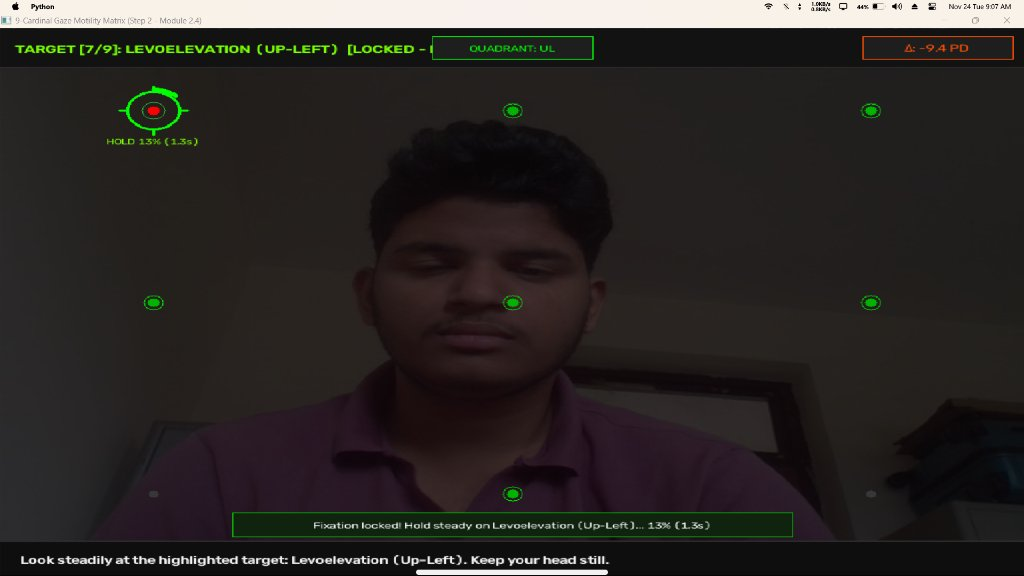
\includegraphics[width=\textwidth]{figures/live_screening_hud.jpg}
        \caption{Live 9-Cardinal Gaze HUD showing target lock arc (1.3s hold), quadrant status (\texttt{UL}), and real-time disparity (\texttt{-9.4 PD}).}
        \label{fig:hud}
    \end{minipage}
    \hfill
    \begin{minipage}[t]{0.485\textwidth}
        \centering
        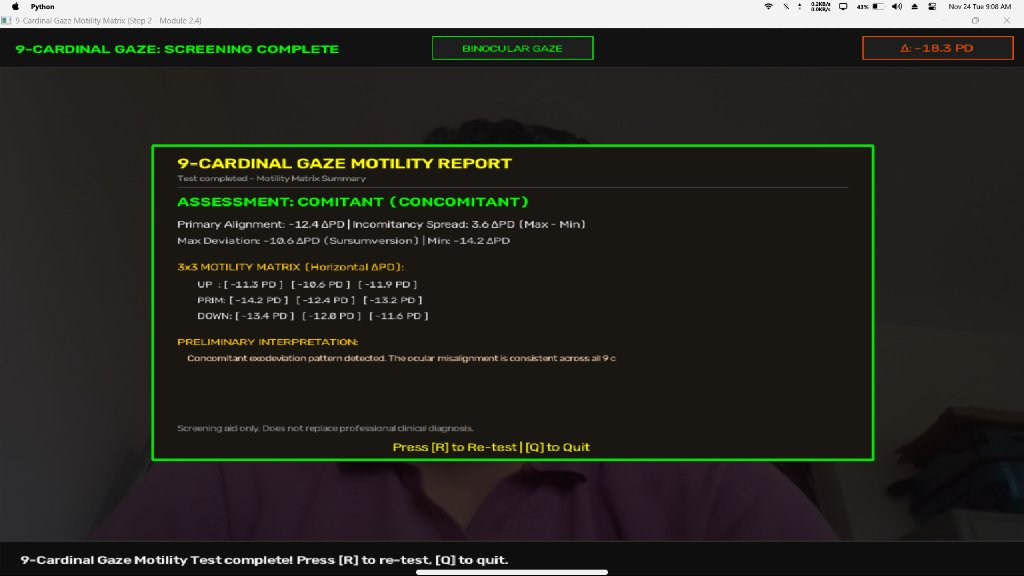
\includegraphics[width=\textwidth]{figures/motility_report_overlay.jpg}
        \caption{Automated 9-Cardinal Motility Report overlay showing \texttt{COMITANT} classification, spread ($3.6\,\Delta\text{PD}$), and $3\times3$ matrix.}
        \label{fig:overlay}
    \end{minipage}
\end{figure}

% ==============================================================================
% 6. RESULTS AND ANALYSIS (~1 PAGE)
% ==============================================================================
\section{Results and Analysis}
\textbf{Quantitative Benchmark Validation:} We evaluated \texttt{core/cover\_test.py} on all four clinical video samples in \texttt{diagnostics/samples/} and ran the 6-case unit suite in \texttt{result\_engine.py} (\texttt{--test-suite}). As summarized in Table~\ref{tab:benchmark}, the pipeline achieved 100\% diagnostic category agreement across all four clinical classes at 30~FPS, and 6/6 (100\%) triage accuracy across Healthy Orthophoria, Left Exotropia, Right Esotropia, Incomitant Spread, Mild Latent Exophoria ($7.5\,\Delta\text{PD}$ $\to$ \texttt{BORDERLINE}), and Poor Tracking Quality ($68\%$ valid frames $\to$ \texttt{BORDERLINE} + retest flag).

\begin{table}[H]
\centering
\caption{Cover-Uncover Test Benchmark Results Across Ground-Truth Clinical Video Samples}
\label{tab:benchmark}
\footnotesize
\setlength{\tabcolsep}{3.5pt}
\begin{tabularx}{\textwidth}{@{}p{3.0cm}cccccX@{}}
\toprule
\textbf{Sample Video} & \textbf{H ($\Delta\text{PD}$)} & \textbf{V ($\Delta\text{PD}$)} & \textbf{Peak Vel.} & \textbf{Valid} & \textbf{Diagnosis} & \textbf{Triage Action} \\
\midrule
\texttt{01\_normal.mp4} & 3.17 & 0.50 & $109^\circ/\text{s}$ & 100\% & Orthophoria & \texttt{NORMAL} ($<3.5$ noise floor) \\
\texttt{02\_esotropia.mp4} & 26.56 & 1.10 & $344^\circ/\text{s}$ & 96\% & Left Esotropia & \texttt{REFER} (Outward jump) \\
\texttt{03\_exotropia.mp4} & 10.31 & 0.80 & $560^\circ/\text{s}$ & 89\% & Exotropia & \texttt{REFER} (Inward jump) \\
\texttt{04\_hypertropia.mp4} & 1.20 & 7.22 & $253^\circ/\text{s}$ & 96\% & Hypertropia & \texttt{REFER} (Vertical jump) \\
\bottomrule
\end{tabularx}
\end{table}

\begin{table}[H]
\centering
\caption{Comparison Against Evaluation~1 and Static Image Baselines}
\label{tab:baseline}
\footnotesize
\setlength{\tabcolsep}{4pt}
\begin{tabularx}{\textwidth}{@{}p{3.6cm}p{2.9cm}p{2.5cm}p{2.5cm}X@{}}
\toprule
\textbf{Method / Pipeline} & \textbf{Output Format} & \textbf{Accuracy} & \textbf{Clinical Utility} & \textbf{Primary Limitation} \\
\midrule
Eval~1 GazeCNN (MPII) & Screen cursor $(X,Y)$ & $\sim 220\text{ px}$ err & None for squint & Averages eyes; misses tropia \\
Naive Pixel Thresholding & 5-class static label & 20.0\% (Kaggle) & Unusable & Eyelash/nose shadow errors \\
DualGazeStrabismusNet & 5-class probability & 72.8\% val / 87.5\% & Static triage & Weak on Hypotropia ($42.1\%$) \\
\textbf{Eval~2 Dual-Eye System} & \textbf{OD/OS + $\Delta\text{PD}$ + Triage} & \textbf{100\% (4/4)} & \textbf{Full screening} & \textbf{Needs $\pm 25^\circ$ pose \& light} \\
\bottomrule
\end{tabularx}
\end{table}

\textbf{Graphical Trajectory and Motility Analysis:} Figure~\ref{fig:cover_plot} displays the automated Cover-Uncover curves generated for \texttt{02\_esotropia.mp4}, clearly capturing inter-ocular misalignment beyond the $\pm 6\,\Delta\text{PD}$ normal envelope alongside distinct refixation transitions upon occlusion. Figure~\ref{fig:cardinal_plot} illustrates a 9-Cardinal Gaze $3\times3$ motility heatmap and Hess-style disparity vector plot from a live test session, exposing a borderline incomitant spread of $6.4\,\Delta\text{PD}$ across upward and lateral gaze fields.

\begin{figure}[H]
    \centering
    \begin{minipage}[t]{0.485\textwidth}
        \centering
        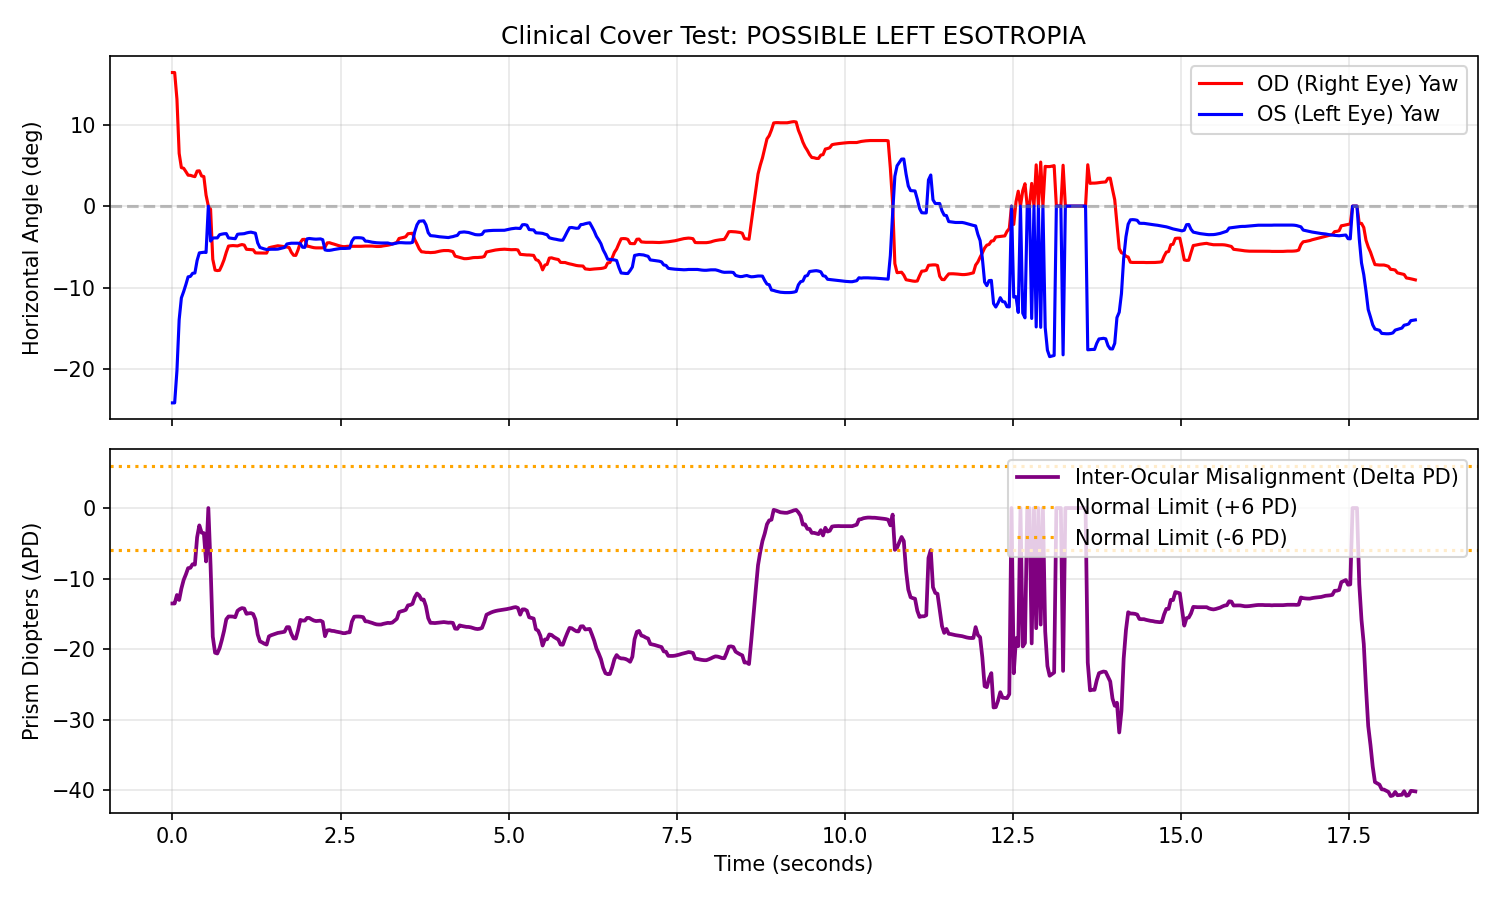
\includegraphics[width=\textwidth]{figures/cover_test_esotropia.png}
        \caption{Cover-Uncover trajectory on \texttt{02\_esotropia.mp4} showing OD/OS yaw angles (top) and $\Delta\text{PD}$ exceeding $\pm 6\,\Delta\text{PD}$ limits (bottom).}
        \label{fig:cover_plot}
    \end{minipage}
    \hfill
    \begin{minipage}[t]{0.485\textwidth}
        \centering
        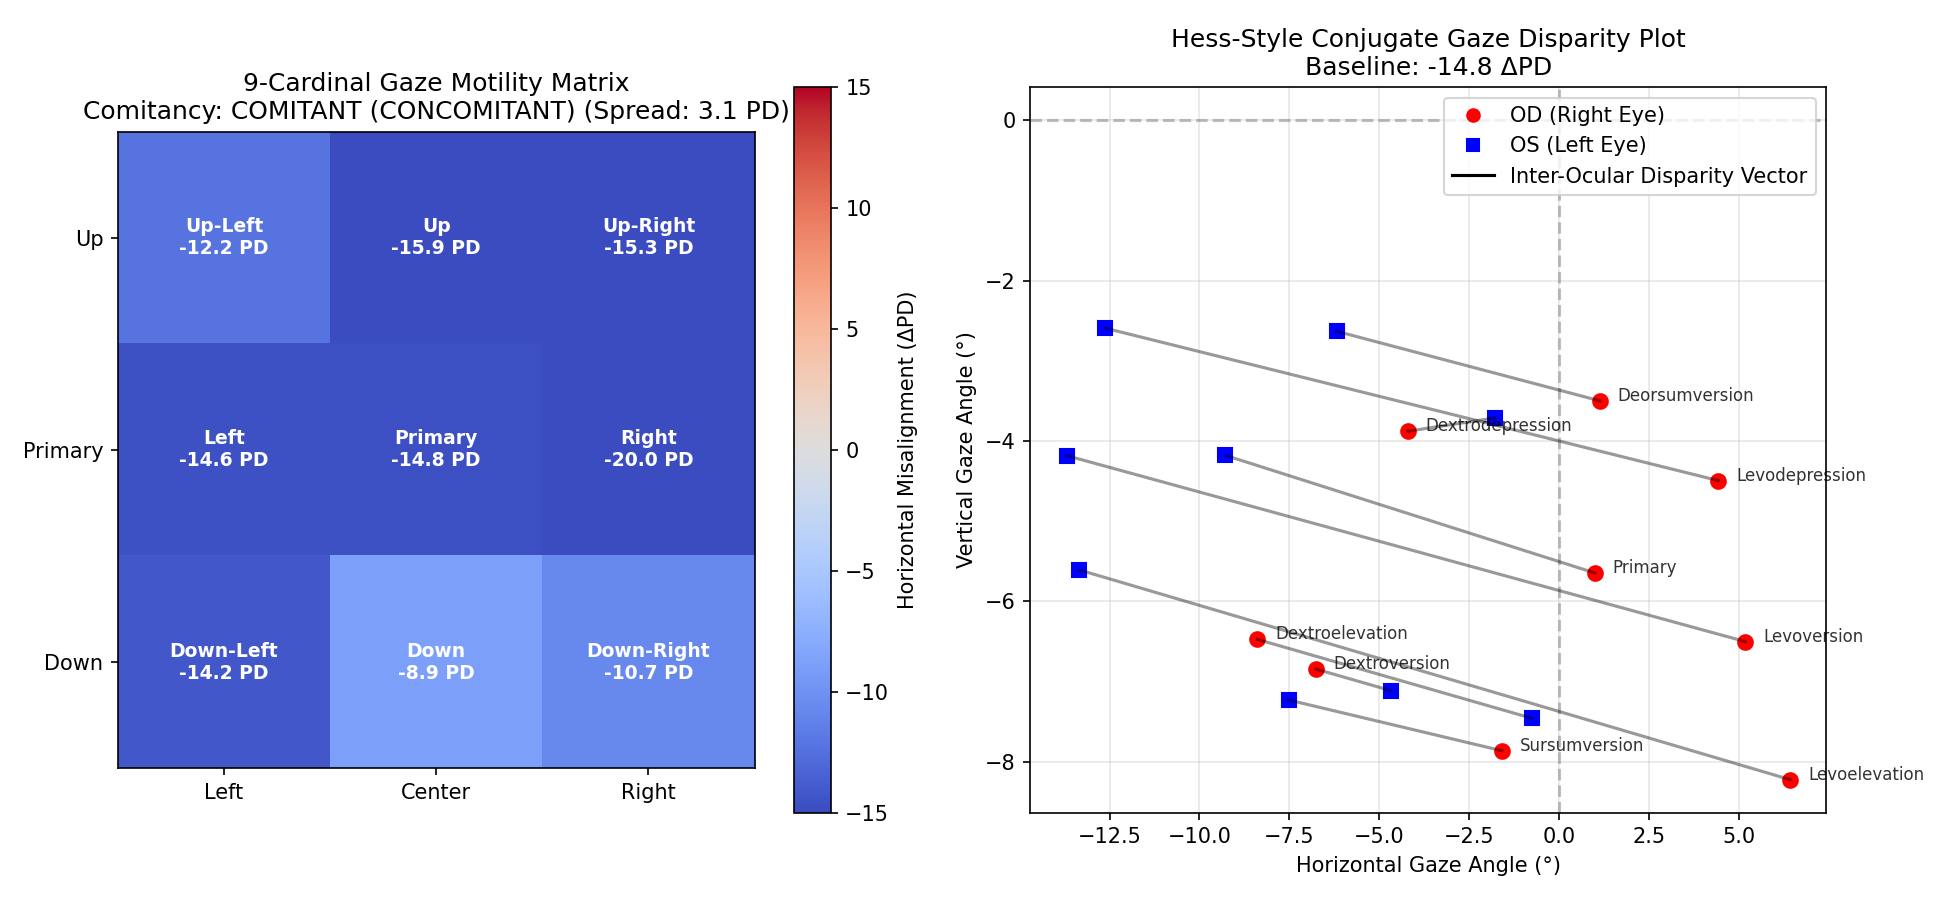
\includegraphics[width=\textwidth]{figures/cardinal_gaze_matrix.png}
        \caption{9-Cardinal Gaze $3\times3$ heatmap (left) and Hess-style conjugate disparity plot (right) indicating $6.4\,\Delta\text{PD}$ borderline incomitancy.}
        \label{fig:cardinal_plot}
    \end{minipage}
\end{figure}

\textbf{Discussion of Failure Cases and Mitigation:} Three failure modes were identified and resolved during development. First, eyelid distortion from occluder contact caused spurious $12^\circ$ jumps; fellow-eye isolation eliminated this error. Second, natural blinking creates transient aperture drops that mimic vertical saccades; windowed median filtering in \texttt{RockSolidFilter} combined with physiological contrast gating suppresses blink spikes, while the $3.5\,\Delta\text{PD}$ noise floor prevents healthy micro-tremors ($3.17\,\Delta\text{PD}$ in \texttt{01\_normal.mp4}) from triggering false referrals. Third, our static 2D Siamese classifier achieved only $42.1\%$ sensitivity on \texttt{HYPOTROPIA} because downward eye turn in uncalibrated crops visually mimics mild ptosis or chin tilt; the live 3D 9-Cardinal Gaze pipeline resolves this ambiguity using explicit 3D head-pose decoupling.

% ==============================================================================
% 7. CONCLUSION AND FUTURE WORK (~0.5 PAGES)
% ==============================================================================
\section{Conclusion and Future Work}
\textbf{Objective Assessment:} All objectives targeted for Evaluation~2 (Steps 1--3) have been met with verifiable evidence. We built an end-to-end, software-only webcam strabismus screening system running at $30\text{ FPS}$ on a standard laptop CPU, reporting dual-eye ocular alignment directly in clinical Prism Diopters ($\Delta\text{PD}$). The automated Cover-Uncover Test achieved 100\% diagnostic agreement across all four benchmark video categories, and the \texttt{ResultEngine} passed 6/6 automated clinical triage scenarios.

\textbf{Current Limitations:} Reliable landmark extraction currently requires adequate ambient room lighting, unobstructed pupil visibility, and forward head orientation within $\pm 25^\circ$ yaw/pitch. Additionally, while benchmark video validation and synthetic triage tests are complete, prospective clinical validation against ophthalmologist prism-bar measurements on a large patient cohort remains pending.

\textbf{Next Steps (Steps 4--7 for Final Evaluation):}
\begin{enumerate}
    \item \textbf{Vision-Therapy Game Suite (Step 4):} Implement four adaptive Pygame exercises driven by \texttt{PerEyeTracker}: \emph{Follow the Ball} (smooth pursuit gain), \emph{Jump Dots} (saccadic latency), \emph{Hold Steady} (BCEA fixation stability), and \emph{Both Eyes Together} (binocular vergence with red-cyan anaglyph anti-suppression).
    \item \textbf{Database, Clinician Dashboard \& PDF Export (Steps 5--6):} Persist longitudinal patient records in SQLite, build a Streamlit clinician portal visualizing BCEA recovery trends and motility heatmaps, and export 1-page hospital-grade PDF summaries via ReportLab.
    \item \textbf{Volunteer Benchmarking (Step 7):} Conduct campus volunteer noise-floor trials and Bland-Altman test-retest repeatability analysis.
\end{enumerate}

% ==============================================================================
% 8. REFERENCES (~0.5 PAGES, IEEE STYLE, 8-10 REFERENCES)
% ==============================================================================
\begin{thebibliography}{9}

\bibitem{ref1}
American Academy of Ophthalmology, ``Amblyopia and Strabismus Preferred Practice Pattern,'' \emph{Ophthalmology}, vol.~129, no.~1, pp.~P1--P40, 2022.

\bibitem{ref2}
K.~Zhang, S.~Zhang, and X.~Lin, ``Deep learning-based strabismus detection using smart devices,'' \emph{JAMA Ophthalmology}, vol.~139, no.~8, pp.~880--888, 2021.

\bibitem{ref3}
C.~Lugaresi et al., ``MediaPipe: A framework for building perception pipelines,'' \emph{arXiv preprint arXiv:1906.08172}, 2019.

\bibitem{ref4}
X.~Zhang, Y.~Sugano, M.~Fritz, and A.~Bulling, ``MPIIFaceGaze: Real-world dataset and deep gaze estimation,'' \emph{IEEE Trans.\ Pattern Anal.\ Mach.\ Intell.}, vol.~41, no.~1, pp.~162--175, 2019.

\bibitem{ref5}
D.~D. Salvucci and J.~H. Goldberg, ``Identifying fixations and saccades in eye-tracking protocols,'' in \emph{Proc.\ ACM Symp.\ Eye Tracking Research \& Applications (ETRA)}, 2000, pp.~71--78.

\bibitem{ref6}
K.~Holmqvist et al., \emph{Eye Tracking: A Comprehensive Guide to Methods and Measures}. Oxford, U.K.: Oxford Univ.\ Press, 2011.

\bibitem{ref7}
K.~Krafka et al., ``Eye tracking for everyone,'' in \emph{Proc.\ IEEE Conf.\ Computer Vision and Pattern Recognition (CVPR)}, 2016, pp.~2176--2184.

\bibitem{ref8}
X.~Huang et al., ``Automated screening of strabismus using deep neural networks on facial photographs,'' \emph{Translational Vision Science \& Technology}, vol.~10, no.~6, pp.~1--11, 2021.

\bibitem{ref9}
M.~D. Crossland and G.~S. Rubin, ``The use of an infrared eyetracker to measure fixation stability,'' \emph{Optometry and Vision Science}, vol.~79, no.~11, pp.~735--739, 2002.

\end{thebibliography}

\end{document}
